\documentclass{article}
\usepackage[utf8]{inputenc}
\usepackage{geometry}
\usepackage{minted}
\usepackage{framed}
\usepackage{float}
\usepackage{fancyhdr}
\usepackage{graphicx}
\usepackage{caption}
\usepackage{subcaption}
\usepackage{url}
\usepackage[colorlinks = true,
            linkcolor = blue,
            urlcolor  = blue,
            citecolor = blue,
            anchorcolor = blue]{hyperref}
\usepackage{mdframed}

% mdframed box setup
\newmdenv{fullframe}
\newmdenv[leftline=false,rightline=false]{topbot}

% command for auto-numbered questions in outline dboxes
\newcounter{QuestionCounter}
\newcounter{SubQuestionCounter}
\counterwithin{SubQuestionCounter}{QuestionCounter}
 
\newcommand{\questionbox}[2]{
\stepcounter{QuestionCounter}
\begin{framed}
\noindent
\textbf{[#1 pts] Problem \arabic{QuestionCounter}}
\vspace{5pt}
\newline
\noindent#2
\end{framed}
}

\newcommand{\nextsubquestionbox}[2]{
\stepcounter{SubQuestionCounter}
\begin{framed}
\noindent\textbf{[#1 pts] Problem \arabic{QuestionCounter}\alph{SubQuestionCounter}}
\vspace{5pt}
\newline
\noindent#2
\end{framed}
}

\newcommand{\firstsubquestionbox}[2]{
\stepcounter{QuestionCounter}
\nextsubquestionbox{#1}{#2}
}

% header setup
\fancyhf{}
\rhead{Spring 2025}
\lhead{CS1430 Programming Assignment 1}
\cfoot{Page \thepage}

\title{CS1430 Programming Assignment 1}
\author{COMPSCI 143}
\date{Spring 2025}

\begin{document}
\pagestyle{plain}
\pagenumbering{gobble}
%\maketitle
%\newpage

\pagestyle{fancy}
\pagenumbering{arabic}


\section{Overview}
In this assignment you will learn the basics of Software Defined Networking (SDN) and a few of its applications.
We will be working with OpenFlow, a communications interface defined between the control and forwarding layers of an SDN architecture.
You will first use a simulator called Mininet to simulate a network topology that uses OpenFlow switches.
Then, you will write the control logic for those switches to manipulate packets.

\subsection{Command Line Interfaces}
We will be working with various command line interfaces:

\begin{enumerate}
    
    \item Commands prefixed with \texttt{\$} are to be run in your VM terminal:
    
    \begin{topbot}
    \begin{minted}[autogobble]{shell-session}
    $ command
    \end{minted}
    \end{topbot}
    
    % \item Commands prefixed with \texttt{\#} are to be run in your terminal using \texttt{sudo} or with root privileges:
    
    % \begin{topbot}
    % \begin{minted}[autogobble]{shell-session}
    % # command
    % \end{minted}
    % \end{topbot}
    
    \item Commands prefixed with \texttt{mininet>} are to be run via the Mininet prompt:
    
    \begin{topbot}
    \begin{minted}[autogobble]{doscon}
    mininet> command
    \end{minted}
    \end{topbot}

    You can enter the Mininet prompt by running \texttt{sudo mn} in your VM terminal.
    
    \item Commands prefixed with \texttt{h1>} are to be run in host \texttt{h1}'s console:
    
    \begin{topbot}
    \begin{minted}[autogobble]{doscon}
    h1> command
    \end{minted}
    \end{topbot}

    You can enter, for example, host \texttt{h1}'s console by running \texttt{xterm h1} at the Mininet prompt.
    Note that the above applies to \texttt{h2}, \texttt{h3}, etc.
    
    % Note: we will prefer not to use root \texttt{\#} and perform all necessary commands using \texttt{sudo}.
    
\end{enumerate}

% \subsection{Dependencies}
% To complete this assignment, you will need the following:
% \begin{itemize}
%     \item Python 3 - \url{https://www.python.org/downloads/}
%     \item Mininet - \url{https://mininet.org/download/}
%     \item POX - \url{https://github.com/noxrepo/pox}
% \end{itemize}
% For some operating systems, such as Mac OS and Linux, Python 3 may already be installed.

\subsection{Python Resources}

% \begin{framed}
%     \noindent
%     \textbf{Note}: Mininet and POX are older software requiring Python 2.7. Please be mindful of slight syntactical differences between modern Python 3 and the older Python 2.
% \end{framed}

Students comfortable with Python may skip this section.
The following resources may be helpful in familiarizing yourself with Python's syntax.

\begin{enumerate}
    \item \url{http://www.codecademy.com/en/tracks/python}
    \item \url{https://docs.python.org/3/tutorial}
\end{enumerate}

% \section{Setting Up Mininet and POX}
% To get started with Mininet, follow the instructions from \url{https://mininet.org/download/}.
% We strongly recommend using their supplied VM options.

\section{VM Setup and Testing}

In this section, you will set up a virtual machine (VM) that runs Mininet and OpenFlow.
To get an idea of what is going on under the hood with Mininet, you may want to consult these two videos:

\begin{enumerate}
\item \url{https://www.youtube.com/watch?v=cuej8DaQOwk}
\item \url{https://www.youtube.com/watch?v=tn1-Pxm0ckc} 
\end{enumerate}

Note: Mininet was still based on Python 2 when these videos were published. 

\subsection{Install and Configure VM Environment}

Follow the instructions in \texttt{CS1430 PA1 VM Instructions.pdf}, which can be found on Canvas or at:\\
\url{https://docs.google.com/document/d/1YMNCfLPM4scre4ZasjDBv6XUDtLbTTpHiVTFi6Dy0tM}

\subsection{Ping Harvard's Web Server!}
With the VM running, SSH into your VM and then verify that it can access the Internet by pinging a known web server: \url{www.harvard.edu}.
The following commands will allow you to easily launch additional terminals as well as ping the server.

\begin{topbot}
\begin{minted}[autogobble]{shell-session}
ssh -X mininet@[Your VM IP here] # run this locally
$ xterm &                        # & detaches a process from the terminal
$ ping -c3 www.harvard.edu
\end{minted}
\end{topbot}

% \begin{topbot}
% \begin{minted}[autogobble]{shell-session}
% $ xterm &                   # '&' detaches a process from the terminal
% $ ping -c3 www.harvard.edu  # ping server
% \end{minted}
% \end{topbot}


\questionbox{5}{
What did you see?
How many ICMP packets (ping requests) were sent out and replied to successfully by the web server?
How long did the replies for each individual ping request take?
}

\newpage
\section{Getting Started with Mininet}
Mininet is a network emulation platform that creates a virtual OpenFlow network---controller, switches (or routers), hosts, and links---on a single virtual machine.
Take a look at the following tutorial first:
\url{https://github.com/mininet/openflow-tutorial/wiki/Learn-Development-Tools}

\subsection{Deciphering the Network Topology}

First, exit the Mininet prompt, making sure to clean up and clear the configuration using the \texttt{mn -c} command.
As a general rule, you will always want to run a cleanup before deploying any topology.
Next, start a new Mininet session with the default topology.
The default topology consists of a switch (s1) and two connected hosts (h1, h2) as well as a reference OpenFlow Controller.

\begin{topbot}
\begin{minted}[autogobble]{shell-session}
mininet> exit # exit prompt
$ sudo mn -c  # perform cleanup
$ sudo mn     # relaunch Mininet with default
mininet> h1 ping -c3 h2
mininet> h2 ping -c3 h1
\end{minted}
\end{topbot}

\questionbox{5}{
Draw a precise diagram of the default network topology.
Label each node and its network interface(s) correctly with IP addresses as in the figure from:
\url{https://github.com/mininet/openflow-tutorial/wiki/Learn-Development-Tools\#start-network}
}

\section{Something Finnicky with OpenFlow}
Now we will use a new topology.
Run the commands below and think about what the network topology looks like.
You may want to try pinging a few hosts like before.

\begin{topbot}
\begin{minted}[autogobble]{shell-session}
mininet> exit
$ sudo mn -c
$ sudo mn --topo linear,7 --mac --switch ovsk --controller remote
mininet> h1 ping -c3 h7
\end{minted}
\end{topbot}

\firstsubquestionbox{0.5}
{
Does pinging between hosts work?
}

\nextsubquestionbox{4.5}
{
Explain the difference between this topology and the reference one from Problem 2.
If you were able to ping successfully, draw a diagram of the network topology.
If you were unable to ping successfully, explain how you could fix the issue.
}

\subsection{Another Topology!}
Let's look at another type of topology.
Run the commands below and then answer the question that follows.
This Mininet walkthrough might be helpful: \url{http://mininet.org/walkthrough/}


\begin{topbot}
\begin{minted}[autogobble]{shell-session}
mininet> exit
$ sudo mn -c
$ sudo mn --topo tree,depth=2,fanout=2 --mac --switch ovsk
\end{minted}
\end{topbot}

\questionbox{5}
{
Draw a precise diagram of this network topology, labelling each node and its network interface(s) correctly with IP addresses (with same guidelines as before).
}

\section{Getting Started with POX}

In this section, you will use an OpenFlow controller called POX.
You will also learn how to write network applications (e.g., hubs and Layer-2 MAC learning) on POX and run them on a Mininet-based virtual network.
POX is a Python-based SDN controller platform geared towards research and education. For more details, see:
\url{https://noxrepo.github.io/pox-doc/html/}

\subsection{Running a Simple Network}
The network you will use in this section includes three hosts and a switch with an OpenFlow controller (POX):

\begin{figure}[H]
    \centering
    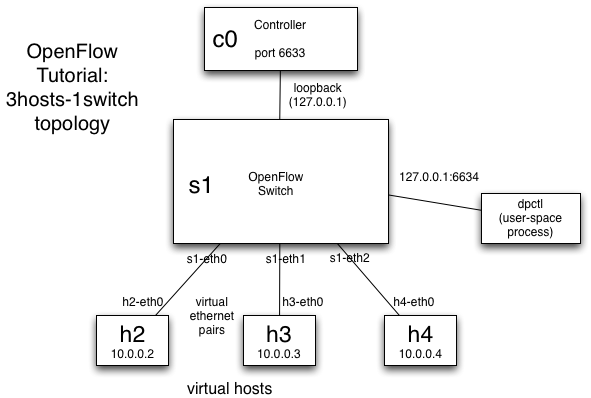
\includegraphics[width=0.5\textwidth]{img/3h_1s.png}
    \caption{Simple network with hosts and a controller.}
    \label{fig:simple_network}
\end{figure}

\pagebreak
Let's get started by cleaning up Mininet and making sure there are no controllers already running on the system.
This is generally good practice, so if you have any bugs or issues, always make sure there are no zombie processes left alive first.
Run the following code:

\begin{topbot}
\begin{minted}[autogobble]{shell-session}
mininet> exit
$ sudo fuser -k 6633/tcp
$ sudo mn -c
\end{minted}
\end{topbot}

Next, we will start both a Mininet virtual network and a POX controller.
You will want to have two terminals for your VM open simultaneously.
To do this, simply open another local terminal and SSH in as usual.
First, let's start up our Mininet virtual network:
\begin{topbot}
\begin{minted}[autogobble]{shell-session}
$ sudo mn --topo single,3 --mac --switch ovsk --controller remote
\end{minted}
\end{topbot}

At this point, the first terminal should show the \texttt{mininet>} prompt.
Note that we have not yet started a controller!
When an OpenFlow switch loses connection to a controller (or starts without one), it will attempt to reestablish contact with the controller, increasing the delay between connection attempts, up to a maximum of 15 seconds.

Next, in your second terminal, let's start a controller for our network to connect to.
Mininet comes with a few basic controllers in the \texttt{pox} directory.
Let's use a basic hub controller that functions by sending all incoming packets out of each of its ports (i.e., to every device it is connected to).
Run the following commands:

\begin{topbot}
\begin{minted}[autogobble]{shell-session}
$ ~/pox/pox.py log.level --DEBUG forwarding.hub
\end{minted}
\end{topbot}

Starting the hub in a verbose debug mode outputs logging information to the terminal, allowing us to see when a switch connects.
At this point, the switches may take some time to connect, generally anywhere between 0 and 15 seconds, as they started without a controller.
If this is too long, the switch may be configured to wait no more than $N$ seconds using the \texttt{--max-backoff} parameter in the future.
For now, you can exit Mininet to remove the switch(es) and then restart Mininet to immediately connect to our already active controller.
Wait until the application indicates that the OpenFlow switch has connected. POX will print a message similar to this:

\begin{topbot}
\begin{minted}[autogobble]{text}
INFO:openflow.of_01:[Con 1/1] Connected to 00-00-00-00-01
DEBUG:samples.of_tutorial:Controlling [Con 1/1]
\end{minted}
\end{topbot}

Note: to avoid delays, you can start the POX controller \textit{before} initializing the Mininet network.

\subsection{Testing the Hub Controller}

Now, verify all hosts can ping each other and see the exact same traffic---the expected behavior of a hub.
We will need to be able to run command to control and view the traffic in each host.
In the Mininet console, run the following to start up the separate xterms (console windows):

\begin{topbot}
\begin{minted}[autogobble]{doscon}
mininet> xterm h1 h2 h3
\end{minted}
\end{topbot}

\pagebreak
\noindent
Arrange the terminals so you can see all of them simultaneously.
It may look something like this:

\begin{figure}[H]
    \centering
    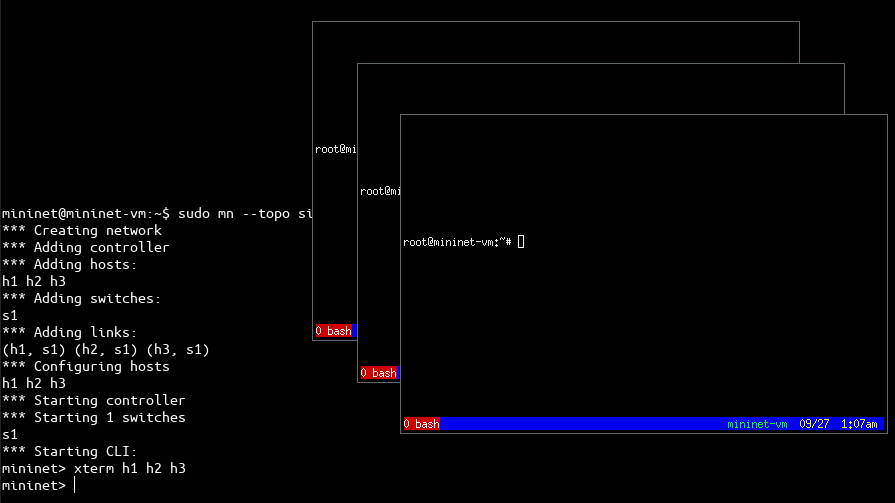
\includegraphics[width=0.75\textwidth]{img/3_xterms.png}
    \caption{Mininet prompt with multiple xterm windows open.}
    \label{fig:3_xterms}
\end{figure}

To inspect traffic, we will use a utility called \texttt{tcpdump}, which prints the packets a host receives on a specified network interface.
Run the following commands \textit{in order} (double-check the prefixes and take note of which host each command is run onr):

\begin{topbot}
\begin{minted}[autogobble]{doscon}
h2> tcpdump -XX -n -i h2-eth0 # run tcpdump on h2
h3> tcpdump -XX -n -i h3-eth0 # run tcpdump on h3
h1> ping -c1 10.0.0.2         # ping from h1
\end{minted}
\end{topbot}

\firstsubquestionbox{2.5}
{
You should see two types of packets in the \texttt{tcpdump} output on the xterms of h2 and h3.
What are the two types?
Draw the path of ping packets on a diagram of the network (both request and response packets).
}

\nextsubquestionbox{2.5}
{
Now, see what happens when a non-existent host fails to reply (e.g., \texttt{ping -c1 10.0.0.5}).
How many packets and of what type do you see in the \texttt{tcpdump} output for h2 and h3?
}

\subsection{Benchmarking the Hub}

Now we will perform some benchmarking of the network topology and hub controller.
For now, we simply want to test how much data a hub can handle.
Luckily, there is a nice tool called \texttt{iperf} that can help us.
Run the following commands on the console with the Mininet prompt:

\begin{topbot}
\begin{minted}[autogobble]{doscon}
mininet> pingall  # verify all nodes are reachable
mininet> iperf    # perform the benchmark
\end{minted}
\end{topbot}

\nextsubquestionbox{2.5}
{
What sort of speeds are you seeing?
The virtual links in Mininet have a very high bandwidth, so they should not be a bottleneck/reason for slow speeds.
Based on what you now know about OpenFlow and this hub, can you give a few reasons for why speeds may be slower than expected?
}

\subsection*{Quick Note: Hub Code}
You can look at the hub code provided by Mininet and POX at \nolinkurl{~/pox/pox/forwarding/hub.py}.
This will be useful for the next few sections.

\section{Switch Controller}
This time, let's verify that hosts can ping each other when the controller is behaving like a Layer-2 learning switch.
Kill the POX controller by pressing Ctrl-C (or Cmd-C) in the terminal running the controller program.
We can launch the L2 learning switch and utilize the 3 xterms from before.
To set things up, first start the controller and network in separate windows:

\begin{topbot}
\begin{minted}[autogobble]{shell-session}
$ sudo mn --topo single,3 --mac --switch ovsk --controller remote
$ pox.py log.level --DEBUG forwarding.l2_learning # starting the learning switch!
\end{minted}
\end{topbot}

Launch xterms for the Mininet hosts and run the commands as we did previously:
\begin{topbot}
\begin{minted}[autogobble]{doscon}
mininet> xterm h1 h2 h3
h2> tcpdump -XX -n -i h2-eth0
h3> tcpdump -XX -n -i h3-eth0
h1> ping -c1 10.0.0.2
\end{minted}
\end{topbot}

\questionbox{5}{
What do you see?
Examine the code of the L2 learning controller at\newline
\nolinkurl{~/pox/pox/forwarding/l2_learning.py}.
Explain the behavior of this controller.
}

\subsection*{Additional Material}
The POX Wiki at \url{https://noxrepo.github.io/pox-doc/html/} can give you a complete tour---skim the wiki if you have any questions.

\section{Programming Custom Network Topology}
In this section, you will learn how to build a custom topology using the Mininet Python API and how parameters such as bandwidth, delay, loss, and queue size can be set individually for different links in the topology.
You will also learn how to test the performance of a topology using \texttt{ping} and \texttt{iperf}.
After the overview, you will create your own custom topology based on a common 3-tier datacenter architecture (i.e., core, aggregation, and edge).
Make sure to follow each step carefully.

\subsection{Overview}

The network you will use in this exercise connects hosts and switches in a linear topology as shown:

\begin{figure}[H]
    \centering
    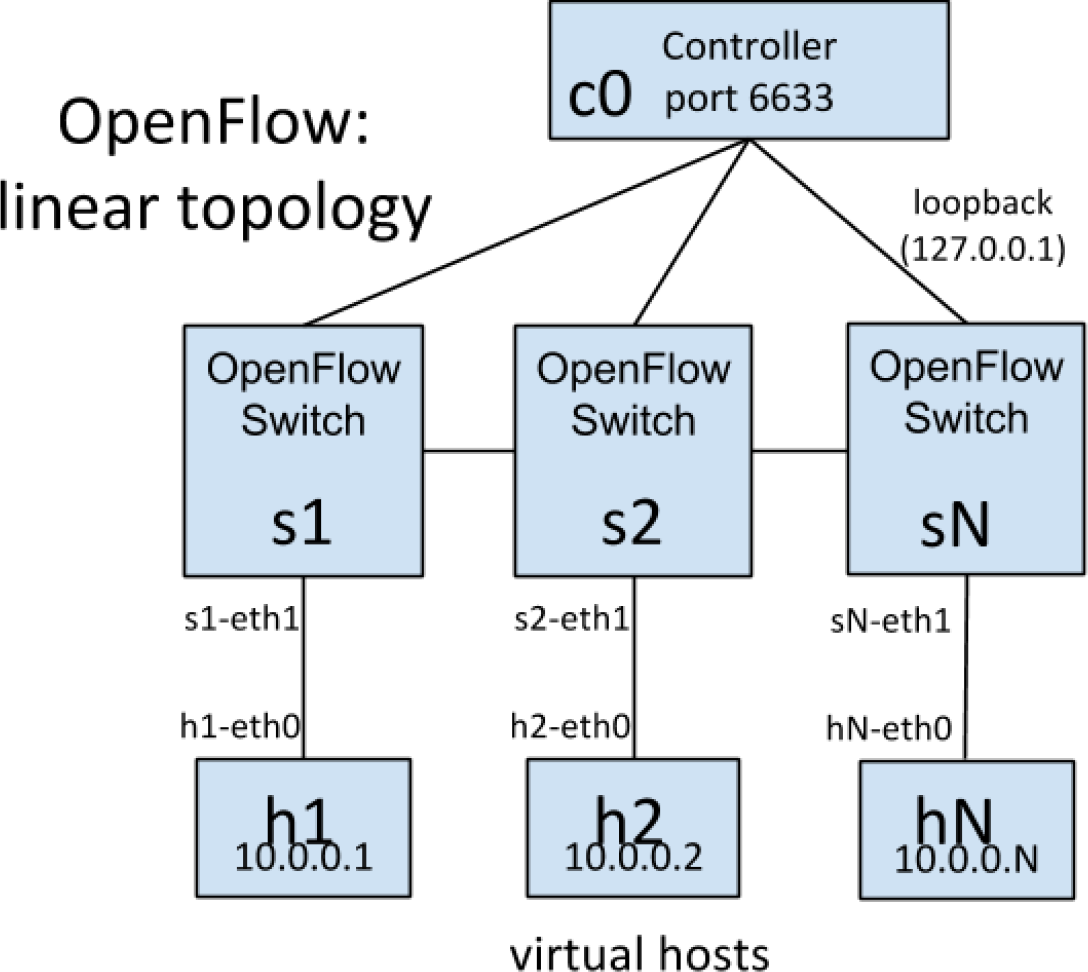
\includegraphics[width=0.5\textwidth]{img/linear_topology.png}
    \caption{Linear network topology.}
    \label{fig:linear_topology}
\end{figure}

\noindent
The code for this topology can be found in the assignment folder as \nolinkurl{topologies/LinearTopo.py} as well as on the following page:

\newpage
\inputminted[fontsize=\footnotesize]{python}{topologies/LinearTopo.py}
\newpage
\noindent
The important classes, methods, functions, and variables in the above code include:

\begin{itemize}
    \item \mintinline{python}{Topo}: the base class for Mininet topologies
    \item \mintinline{python}{addSwitch(name)}: add a switch to the topology and return the switch name
    \item \mintinline{python}{addHost(name)}: add a host to the topology and return the host name
    \item \mintinline{python}{addLink(a, b)}: add a bidirectional link to the topology (and return the link key)\\
    Note: Links in Mininet are bidirectional unless noted otherwise.
    \item \mintinline{python}{Mininet}: main class to create and manage a network
    \item \mintinline{python}{start()}: start the network
    \item \mintinline{python}{pingAll()}: test connectivity by having all nodes ping each other
    \item \mintinline{python}{stop()}: stop the network
    \item \mintinline{python}{net.hosts}: all hosts in the network\\
    Note: this is an instance attribute; in our case, \texttt{net} is the \texttt{Mininet} class instance.
    \item \mintinline{python}{setLogLevel(level)}: set Mininet's default output level\\
    Note: valid levels are: \texttt{`info' | `debug' | `output'}
\end{itemize}

\subsection{Setting Performance Parameters}
In addition to basic behavioral networking, Mininet provides performance limiting and isolation features through abstractions such as the \texttt{CPULimitedHost} and \texttt{TCLink} classes.
The code for this topology can be found in the assignment folder as \nolinkurl{topologies/LinearTopoPerf.py} as well as on the following page:

\newpage
\inputminted[fontsize=\footnotesize]{python}{topologies/LinearTopoPerf.py}
\newpage

\subsection{Running the Custom Topologies}
To run the custom topology above, download \textbf{LinearTopo.py}.

\begin{topbot}
\begin{minted}[autogobble]{shell-session}
$ cd ~
$ chmod u+x LinearTopo.py
$ sudo ./LinearTopo.py
\end{minted}
\end{topbot}

\noindent
To run the topology with performance parameters, use \textbf{LinearTopoPerf.py} instead.

\subsection{Programming a Datacenter Network Topology}
Datacenter networks typically have a tree-like topology.
End hosts connect to top-of-rack switches, which form the leaves (edges) of the tree.
One or more core switches form the root, and one or more layers of aggregation switches form the middle of the tree.
In a basic tree topology, each switch (except the core switch) has a single parent.
Additional switches and links may be added to form more complex topologies (e.g., fat tree) to improve fault tolerance or increase total bandwidth.

In this section, your task will be to create a simple tree topology.
You will assume each level (i.e. core, aggregation, edge, and host) to be composed of a single layer of switches and hosts with a configurable fanout value ($k$).
For example. a simple tree network having a single layer per level with fanout $k = 2$ looks like:

\begin{figure}[H]
    \centering
    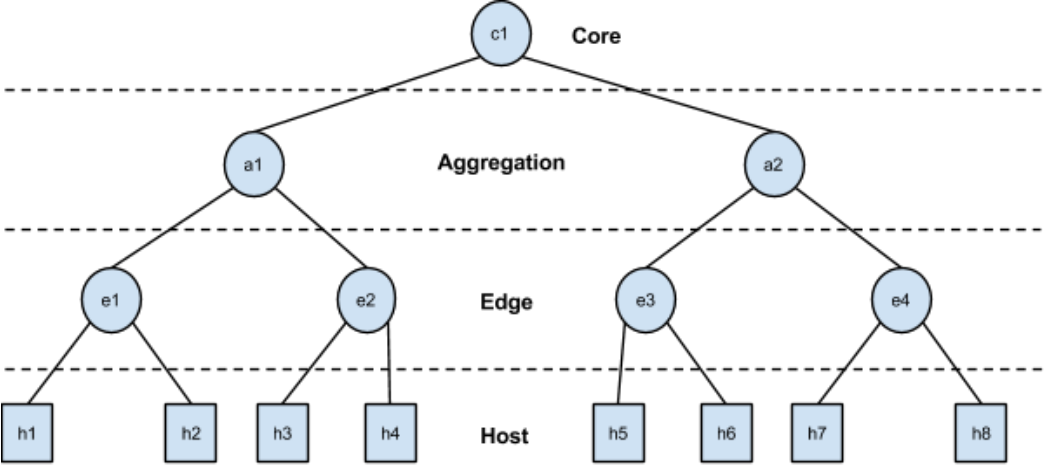
\includegraphics[width=0.6\textwidth]{img/dc_topology.png}
    \caption{Datacenter tree topology.}
    \label{fig:dc_topology}
\end{figure}

\noindent
To begin, download and unzip \texttt{q7.zip}.
The file \texttt{CustomTopo.py} contains a template which takes the following arguments as input:

\begin{itemize}
    \item \texttt{linkopts1}: performance parameters for links between core and aggregation switches
    \item \texttt{linkopts2}: performance parameters for links between aggregation and edge switches
    \item \texttt{linkopts3}: performance parameters for links between edge switches and hosts
    \item \texttt{fanout}: fanout degree (children per node)
\end{itemize}

\questionbox{5}{
Create the tree-based datacenter topology described above.
Your logic should support setting at least the \texttt{bw} and \texttt{delay} parameters for each link.
}

\subsection{Testing Your Code}
Edit \texttt{CustomTopo.py} to pass in \texttt{linkopts1}, \texttt{linkopts2}, and \texttt{linkopts3} when the class is instantiated.
You may uncomment the sample code and link options we provide to test the topology:

\begin{topbot}
\begin{minted}[autogobble]{python}
linkopts1 = dict(bw=10, delay="5ms", loss=10, max_queue_size=1000, use_htb=True)
linkopts2 = dict(bw=10, delay="5ms", loss=10, max_queue_size=1000, use_htb=True)
linkopts3 = dict(bw=10, delay="5ms", loss=10, max_queue_size=1000, use_htb=True)
topos = { "custom": ( lambda: CustomTopo(linkopts1,linkopts2,linkopts3) ) }
\end{minted}
\end{topbot}

\noindent
Run the Mininet ping test with the custom topology:

\begin{topbot}
\begin{minted}[autogobble]{shell-session}
$ sudo mn --custom CustomTopo.py --topo custom --test pingall --link tc
\end{minted}
\end{topbot}

\noindent
If everything has been set up correctly, you should observe the behavior specified by the link options provided.
Feel free to adjust the parameters shown above (e.g., \texttt{bw}, \texttt{delay}, \texttt{loss}) to see what effects they may have.

\section{Layer 2 Firewall}

In this section, you will create a network application that implements a Layer 2 firewall.
This firewall selectively disables inbound and outbound traffic between two systems based on their MAC address.

\subsection{Overview}
A firewall is a network security system that is used to control the flow of ingress and egress traffic---usually between a more secure local-area network (LAN) and a less secure wide-area network (WAN).
The system analyzes packets for parameters such as L2/L3 headers (i.e., MAC and IP) or performs deep packet inspection (DPI) for higher layers (e.g., application type, services, etc.) to filter network traffic.

POX allows running multiple applications concurrently (e.g., MAC learning in conjunction with firewalling), but it does not automatically handle rule conflicts.
You have to ensure that conflicting rules are not being installed by multiple applications (e.g., both applications trying to install rules with the same source and destination MACs at the same priority level but with different actions).
The most simplistic way to avoid this contention is to assign different priority levels to each application.

\subsection{Programming a Firewall}
In this section, your task is to implement a Layer 2 firewall that runs alongside the MAC learning module on the POX OpenFlow controller.
The firewall will be provided a list of MAC address pairs in the form of an access control list (ACL).
When a connection establishes between the controller and the switch, the application installs flow rule entries in the OpenFlow table to disable all communication between the specified MAC pairs.
Your firewall should be agnostic of the underlying topology and should take a MAC pair list as input to install rules on the switches.
To make things easier, we will simply install the rules on \textbf{all} switches in the network.

\noindent
To get started, download and unzip \texttt{q8.zip}.
You should see:

\begin{itemize}
    \item \texttt{firewall.py}: a skeleton class you will update with logic for installing firewall rules.
    \item \texttt{firewall-policies.csv}: list of MAC pairs (policies) read as input by the firewall.
\end{itemize}

The policy list (\texttt{firewall-policies.csv}) specifies MAC addresses that are not permitted to communicate with each other.
You will not need to modify the policy list.
The skeleton class inside \texttt{firewall.py} contains a function named \texttt{\_handle\_ConnectionUp()}.
The file also contains a global variable, \texttt{policyFile}, that should hold the path of \texttt{firewall-policies.csv}.
Whenever a connection is established between the POX controller and the OpenFlow switch, \texttt{\_handle\_ConnectionUp()} is called.

\questionbox{5}{
Update the \texttt{\_handle\_ConnectionUp()} function to install rules for the OpenFlow switches so that they drop any incoming packet containing a source and destination MAC address pair forbidden by our policy list. (Note: make sure to handle any conflicts carefully---we will be testing with different policy lists!)
%Write a function that reads the policy file and update the \_handle\_ConnectionUp function. The function should install rules in the OpenFlow switch that drop packets whenever a matching src/dst MAC address (for any of the listed MAC pairs) enters the switch. (Note: make sure that you handle the conflicts carefully.)
}

\subsection{Testing Your Code}
Copy \texttt{firewall.py} and \texttt{firewall-policies.csv} into \nolinkurl{~/pox/pox/misc} on your VM.
The rule shown below disables all communication between hosts h1 and h2:
\begin{topbot}
\begin{minted}[autogobble]{text}
id,mac_0,mac_1
1,00:00:00:00:00:01,00:00:00:00:00:02
\end{minted}
\end{topbot}

\noindent
With this rule in place, let's see what happens when we attempt to ping one host from the other.
Take note that we are invoking the POX controller command with an ampersand suffix (\texttt{\&}), which will start the process in the background and allow us to continue using the same terminal for additional commands.
Alternatively, you may choose to run the POX controller and Mininet commands in separate terminals.

\begin{topbot}
\begin{minted}[autogobble]{shell-session}
$ cd ~
$ sudo fuser -k 6633/tcp
$ pox.py forwarding.l2_learning misc.firewall &     # start POX controller
$ sudo mn --topo single,3 --controller remote --mac # deploy Mininet topology
mininet> h1 ping -c1 h2 # ping h2 from h1
\end{minted}
\end{topbot}

If everything has been set up correctly, you should see that neither host h1 nor host h3 are able to successfully ping host h2.
However, host h1 should still be able to ping host h3 (and vice versa) since there is no flow rule installed that forbids communication between the two.

\section{Custom OpenFlow Controller - Dijkstra's Algorithm}
In this section, you will utilize Dijkstra's algorithm to find the shortest path between every pair of nodes.
You will then write an OpenFlow controller that leverages the algorithm to dynamically create its own routing table.

\subsection{Getting Started}
To get started, download and unzip \texttt{q9.zip}.
You will see the following files:

\begin{itemize}
    \item \texttt{topo.py}: a skeleton class you will update with logic for creating the network topology with custom delays shown below
    \item \texttt{dijkstra.py}: a skeleton class you will update with shortest-path routing logic
    \item \texttt{delay.csv}: a list of link, delay value pairs to be read by the controller
\end{itemize}
We will use a specific topology and set of delays as depicted in Figure \ref{fig:custom_topo}. The delay values in the table are from \texttt{delay.csv}.

\begin{figure}[H]
     \centering
     \begin{subfigure}[c]{0.6\textwidth}
         \centering
         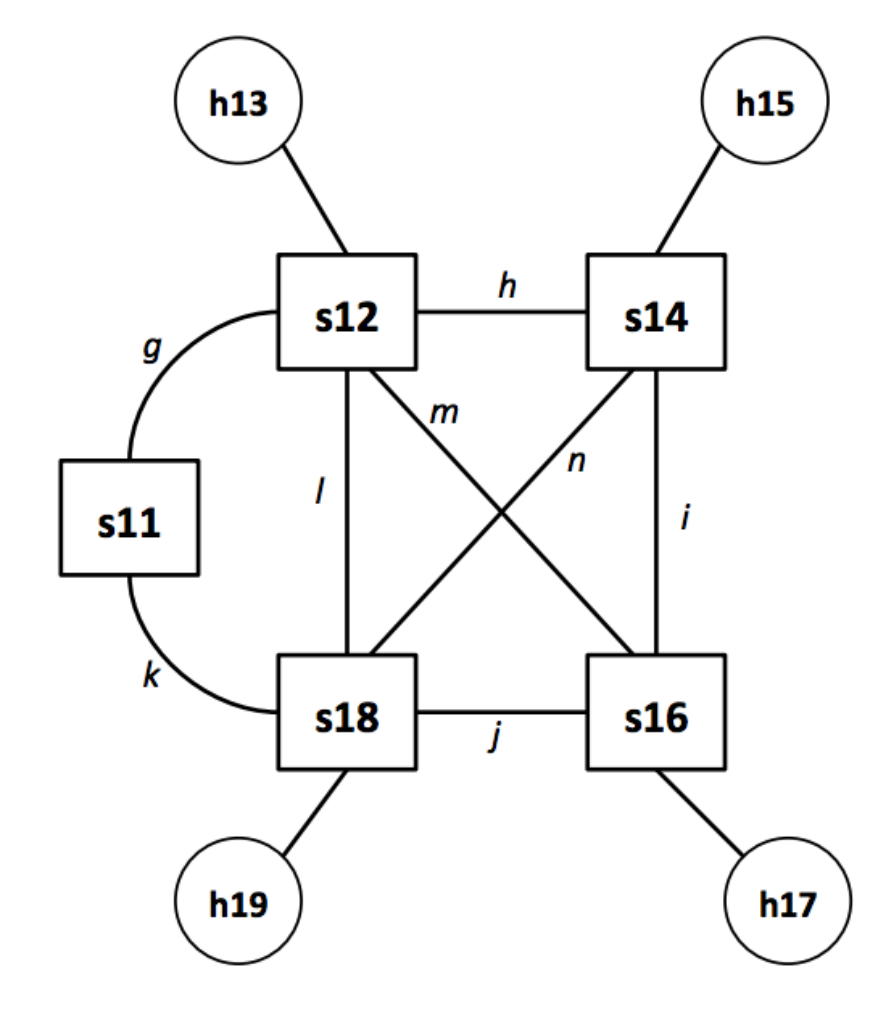
\includegraphics[width=\textwidth]{img/delay_topo.png}

     \end{subfigure}
     \begin{subfigure}[c]{0.3\textwidth}
         \centering
        \begin{tabular}{cc}
            \hline
            Link & Delay(ms) \\
            \hline
            g & 10 \\
            h & 50 \\
            i & 10 \\
            j & 30 \\
            k & 30 \\
            l & 10 \\
            m & 100 \\
            n & 20 \\
            \hline
        \end{tabular}
     \end{subfigure}
     \caption{Custom topology and delay table}
     \label{fig:custom_topo}
\end{figure}

\firstsubquestionbox{5}{
Implement the topology depicted in Figure \ref{fig:custom_topo} in \texttt{topo.py}.
}

\nextsubquestionbox{5}{
Factoring in the delays shown for each link, manually determine the ``shortest'' paths (i.e., those with the least delay) for each pair of hosts in the topology.
Which nodes are in each shortest path and how much time does each path require?
Note: use Dijkstra's algorithm.
}

\nextsubquestionbox{5}{
Write pseudocode for your controller using Dijkstra's algorithm to find the shortest paths between all pairs of nodes given a topology and link delay table.
You may assume that a dictionary mapping link labels to delay values exists (such as in \texttt{delay.csv}).
}

\nextsubquestionbox{5}{
Implement your code in \texttt{dijkstra.py}.
Notice that the filename \texttt{delay.csv} is assigned to the variable \texttt{delayFile}.
You may assume a static topology shape and hard-code link labels (e.g., $g$, $h$, $i$, etc.), but \textbf{do not} hard-code the delays: your implementation must be general enough to function properly even with different delay values.
}

\subsection{Testing your Code}
Once you have your code, copy \texttt{dijkstra.py} and \texttt{delay.csv} into the \nolinkurl{~/pox/pox/misc} directory on your VM.
Run the following commands to see your code in action:

\begin{topbot}
\begin{minted}[autogobble]{shell-session}
$ cd ~/pox/pox/misc/
$ pox.py misc.dijkstra &
$ sudo mn --custom topo.py --topo custom --controller remote --mac --link tc
\end{minted}
\end{topbot}

In Mininet, try pinging host (h17) from host (h13).
If everything has been set up correctly, host (h13) will ping (h17), showing a RTT corresponding to the shortest path you  earlier.
You may wish to additionally ping between each pair of hosts to validate your results.

\newpage
\section{Submitting the Assignment}
Your submission should be a \texttt{.zip} archive with a \texttt{CS1430\_PA1\_} prefix followed by each team member's full name separated with two underscores from the next name.
Only one submission per team is needed.
The archive should contain:
\begin{itemize}
    \item PDF write-up
    \item Assignment code
    \item README file
\end{itemize}

\noindent
Example filename: \texttt{CS1430\_PA1\_Jane\_Doe\_\_John\_Doe\_\_Jane\_Smith\_\_John-Paul\_Smith.zip}\\

\subsection*{Write-up}
Written responses (and any sketches, diagrams, and screenshots) should be contained within a single PDF document.
(\LaTeX~is highly recommended!)
Each response or figure should clearly indicate which problem is being answered.
The write-up must contain the full names of all team members.

\subsection*{Code}
Code should be organized in directories indicating the question they are for.
You should include \textbf{all} files that were provided, but with the changes you made.
You may choose to follow our naming scheme (e.g., \nolinkurl{q7/}) or use your own, but it should be apparent which files are for which problem.

\subsection*{README}
The README should contain instructions on how to run code you submit (assuming we use the same starting VM image).
Make sure to include details about: where files should be placed, what commands should be run, etc.
The README must also contain the full names of all team members.

\subsection*{Example}
An example submission might look like this:

\begin{figure}[H]
    \centering
    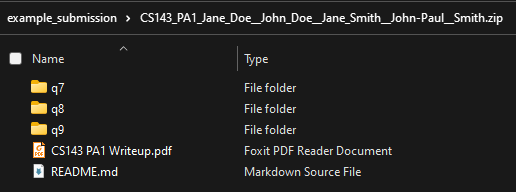
\includegraphics[width=0.5\textwidth]{img/example_submission2.png}
    \caption{Example submission.}
    \label{fig:example_submission}
\end{figure}


\subsection*{Congratulations!}
Congratulations on completing your assignment!
\end{document}
